\documentclass[10pt, a4paper,spanish]{article}

\usepackage[utf8]{inputenc}
\usepackage[spanish]{babel}

\usepackage[T1]{fontenc}

\usepackage[hmarginratio=1:1,top=32mm,columnsep=20pt]{geometry}
\usepackage[hang, small,labelfont=bf,up,textfont=it,up]{caption}

\usepackage{float}

\usepackage{amsmath}

\usepackage{graphicx}
\graphicspath{ {images/} }

\usepackage[hidelinks]{hyperref}

\usepackage{minted}
\usepackage{float}
\RecustomVerbatimEnvironment{Verbatim}{BVerbatim}{}


\usepackage{abstract}
\renewcommand{\abstractnamefont}{\normalfont\bfseries}
\renewcommand{\abstracttextfont}{\normalfont\small\itshape}


\usepackage{titlesec}
\renewcommand\thesection{\Roman{section}}
\renewcommand\thesubsection{\Roman{subsection}}
\titleformat{\section}[block]{\large\scshape\centering}{\thesection.}{1em}{}
\titleformat{\subsection}[block]{\large}{\thesubsection.}{1em}{}

\usepackage{fancyhdr}
\pagestyle{fancy}
\fancyhead{}
\fancyfoot{}
\fancyhead[C]{ \today \ $\bullet$ Minería de Datos $\bullet$ Redes de Elman y Jordan}
\fancyfoot[RO]{\thepage}

%-------------------------------------------------------------------------------
%	TITLE SECTION
%-------------------------------------------------------------------------------

\title{\vspace{-15mm}\fontsize{24pt}{10pt}\selectfont\textbf{Redes de Elman y Jordan}} % Article title

\author{García Prado, Sergio}
\date{\today}

%-------------------------------------------------------------------------------

\begin{document}

	\maketitle % Insert title

	\thispagestyle{fancy} % All pages have headers and footers


%-------------------------------------------------------------------------------
%	ABSTRACT
%-------------------------------------------------------------------------------

	\begin{abstract}
		\noindent Este trabajo consiste en el estudio de las redes neuronales recurrentes (RNN) de \emph{Elman} y \emph{Jordan}. En este documento se describen las fases de dichos algoritmos así como las diferencias entre ellos. Además, se ha realizado una implementación en el lenguaje \emph{Octave} basada en la aproximación a una función temporal de valores escalares procedentes de los resultados de cotización en bolsa de una empresa.
	\end{abstract}

%-------------------------------------------------------------------------------
%	TEXT
%-------------------------------------------------------------------------------


  \section{Introducción}

    \paragraph{}
		Las \textbf{redes neuronales} consisten en una técnica, que se basa en una gran conjunto de neuronas artifiales. Cada unidad neuronal está conectada con otras de una determinada manera. Estos enlaces pueden poseer una función de combinación. Cada neurona puede tener una función encargada de combinar los valores de su entrada. Además, puede haber una función de activación en cada enlace o en la propia neurona: de tal manera que la señal debe superar el límite antes de la propagación hacia otras. Estos sistemas tienen capacidad de  autoaprendizaje. Esto se ilustra gráficamente en la figura \ref{fig:neural-network}.

		\begin{figure}[htpb!]
			\begin{center}
				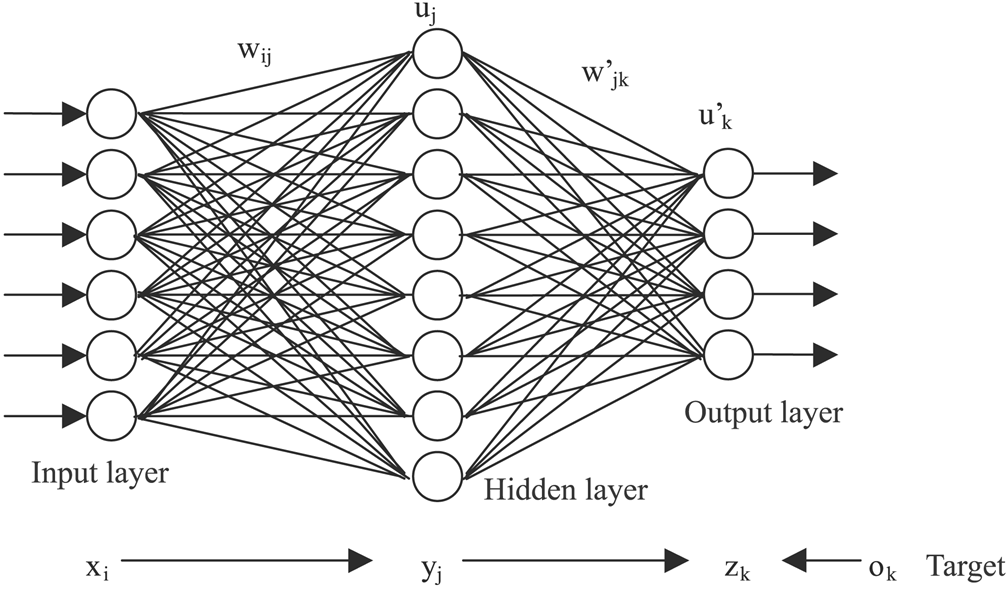
\includegraphics[width=0.75\textwidth]{neural-network}
						\caption{Topología de una red neuronal.}
						\label{fig:neural-network}
				\end{center}
		\end{figure}

		\paragraph{}
		En este documento se va a profundizar en las \textbf{redes neuronales recurrentes}. Estas son un tipo concreto de redes neuronales cuya principal característa es la interconexión recurrente de neuronas. Esto significa que una neurona puede poseer ciclos con otras neuronas, o incluso con ella misma. Esta idea fue desarrollada por \emph{Jordan} en \emph{Serial Order: A parallel distributed approach}(1986)\cite{jordan:article} y por \emph{Elman} en \emph{Finding structure in time}(1990)\cite{elman:article}.

		\paragraph{}
		Por otro lado, el conjunto de datos que se ha utilizado como ejemplo consiste en un conjunto de 254 casos correspondientes a los valores de cotización en bolsa de la empresa \textbf{Iberdrola} durante un periodo de 12 meses (Noviembre de 2015 - Diciembre de 2016). En este fichero aparecen vaios campos, a pesar de ello nos hemos centrado únicamente en el valor de \emph{Cierre}, que es el que se ha utilizado como entrada para la red neuronal.


	\section{Redes de Elman y Jordan}

		\paragraph{}
		En sus respectivos artículos, tanto \emph{Elman} como \emph{Jordan} proponen una red neuronal con estructura de \textbf{3 capas} correspondiendose la primera a la \emph{capa de entrada}, la segunda a la \emph{capa oculta} y la tercera a la \emph{capa de salida}. Además de esto, proponen añadir un conjunto de neuronas (que denominan \emph{capa de contexto}) y las cuales pretenden dotar a la red de capacidad de recuerdo, permitiendo que estas almacenen información acerca de casos anteriores.

		\paragraph{}
		Las diferencias entre estas dos propuestas consisten en la topología de la red, en concreto, en las interconexiones con la \emph{capa de contexto}. Por tanto, la diferencia es la siguiente:

		\begin{itemize}
			\item \textbf{Red de Jordan}: La capa de contexto está conectada con la \textbf{capa de salida}.
			\item \textbf{Red de Elman}: La capa de contexto está conectada con la \textbf{capa oculta}.
		\end{itemize}

		\paragraph{}
		Esto tiene incidencia en las fases de propagación sobre la red (de manera explicita hacia delante y de manera implicita hacia atrás), ya que determina a partir de qué conjunto de neuronas se almacena información en la capa de contexto. Una representación gráfica de estas diferencias se muestra en la figura \ref{fig:topology}

		\begin{figure}[htpb!]
			\begin{center}
				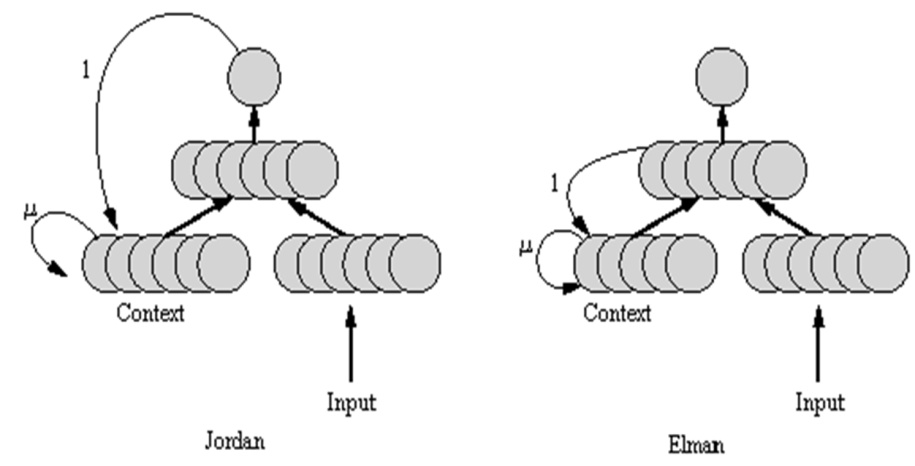
\includegraphics[width=0.75\textwidth]{topology}
						\caption{Topología de las redes neuronales recurrentes de Elman y Jordan.}
						\label{fig:topology}
				\end{center}
		\end{figure}

		\paragraph{}
		Obviando esta diferencia topológica, el resto de la red funciona de la misma forma, por tanto, a continuación se describen el conjunto de pasos que suceden.

		\subsection{Encaminamiento hacia adelante}

			\paragraph{}

		\subsection{Encaminamiento hacia atrás}

			\paragraph{}


	\section{Implementación}

		La sección de implementación se divide en un primer apartado que explica la ejecucción del código de ejemplo seguido de los apartados que explican en detalle cada una de las partes del código fuente


		\subsection{Guía de ejecucción}

			\paragraph{}
			La implementación realizada se ha llevado a cabo en el lenguaje Octave. Se incluyen todos los ficheros de código fuente para poder ejecutar la implementación. Estos se alojan en el directorio \textbf{/src}. Además, se ha añadido un script bash de prueba denominado \textbf{run.sh} el cual permite ejecutar la implementación a partir del terminal si así se desea.

			\paragraph{}
			También se puede iniciar desde el entorno gráfico de Octave asignando el directorio \textbf{/src} como directorio de trabajo y seguidamente llamando a la funcion \textbf{main()}.


		\subsection{Datos de Entrada}

			\paragraph{}
			Tal y como se ha expuesto brevemente al principio de este documento, el conjunto de datos se corresponde con una serie temporal de valores escalares. Además, se indica que tan solo los \textbf{últimos 20 valores} tienen repercusión en el valor próximo que se desea predecir. Este hecho plantea dos enfoques diferentes de entrada hacia la red neuronal:

 			\begin{itemize}
 				\item \textbf{Enfoque Secuencial}: Para cada periodo de aprendizaje o predicción previamente se introducen las 20 muestras previas de manera secuencial para después obtener la siguiente. Esto implica que la red tenga una única neurona en la entrada.

				\item \textbf{Enfoque en Paralelo}: Para cada periodo de aprendizaje o predicción se introducen las 20 muestras previas de una sola vez para después obtener la siguiente. Esto implica que la red tenga tantas neuronas en la entrada como muestras previas relevantes, en este caso 20.
 			\end{itemize}

			\paragraph{}
			Tras realizar pruebas utilizando las dos alternativas no se encontraron diferencias significativas en los resultados obtenidos por ninguna de las dos estrategias, por lo cual se ha optado por el \textbf{Enfoque en Paralelo} debido a la equivalencia de resultados y su menor coste computacional.

			\paragraph{}
			En cuanto a la \emph{capa oculta} se ha escogido un tamaño de \textbf{10 neuronas} basandose en las pruebas realizadas así como en el artículo \emph{Financial Time Series Prediction Using Elman Recurrent Random Neural Networks}\cite{financial:article}.


		\subsection{Normalización}

			\paragraph{}
			La red neuronal está diseñada para trabajar con valores normales (en el rango $[0,1]$) debido a la función sigmoide que se define en el siguiente apartado. Por lo tanto, es necesario realizar una fase previa de normalización de los mismos. Debido a la restricción que indica que la relevancia de sucesos pasados se limita a los 20 últimos casos, se normaliza sobre estos en cada fase del algoritmo.

			Para ello se utilizan las siguientes funciones para normalización y desnormalización, que colapsan el conjunto en torno a su máximo y mínimo:

			\begin{equation}
				S(t)' = frac{S(t) - min S(t)}{max S(t)- min S(t)}
			\end{equation}

			\begin{figure}[htpb!]
				\centering
				\inputminted{octave}{../src/common/normalize.m}
				\caption{Octave: /src/common/normalize.m}
				\label{code:normalize}
			\end{figure}


			\begin{equation}
				S(t) = S(t)' (max S(t)- min S(t)) + min S(t)
			\end{equation}

			\begin{figure}[htpb!]
				\centering
				\inputminted{octave}{../src/common/denormalize.m}
				\caption{Octave: /src/common/denormalize.m}
				\label{code:denormalize}
			\end{figure}

		\subsection{Función Sigmoide}
			\paragraph{}
			La función sigmoide o función de activación es la encargada de determinar el grado de importancia que tendrá un determinado nodo de la red en el valor del siguiente. A continuación se formula la función logística así como su derivada:

			\begin{equation}
				f_H(x) = \frac{1}{1+e^(-x)}
			\end{equation}

			\begin{figure}[htpb!]
				\centering
				\inputminted{octave}{../src/common/sigmoid.m}
				\caption{Octave: /src/common/sigmoid.m}
				\label{code:sigmoid}
			\end{figure}

			\begin{equation}
				\partial f_H(x) = \frac{e^x}{(1 + e^x)^2}
			\end{equation}


			\begin{figure}[htpb!]
				\centering
				\inputminted{octave}{../src/common/dsigmoid.m}
				\caption{Octave: /src/common/dsigmoid.m}
				\label{code:dsigmoid}
			\end{figure}

		\subsection{Inicialización}

			\paragraph{}
			La fase de inicialización se corresponde con la creación de la matriz de capas así como la inicialización de la matriz de pesos, que en este caso se han decido generar aleatoriamente en el rango $[-0.25,0.25]$.

			\paragraph{}
			La función de generación de pesos aleatorios se muestra en la figura \ref{code:random_weights} y es común a los dos métodos (\emph{Elman} y \emph{Jordan})

			\begin{figure}[htpb!]
				\centering
				\inputminted{octave}{../src/common/random_weights.m}
				\caption{Octave: /src/common/random\_weights.m}
				\label{code:random_weights}
			\end{figure}

			\paragraph{}
			Por contra, la generación de la estructura de la red es diferente debido a las diferencias topológicas entre las dos redes.

			\begin{figure}[htpb!]
				\centering
				\inputminted{octave}{../src/elman/elman_generate_layers.m}
				\caption{Octave: /src/elman/elman\_generate\_layers.m}
				\label{code:jordan_generate_layers}
			\end{figure}

			\begin{figure}[htpb!]
				\centering
				\inputminted{octave}{../src/elman/elman_generate_weights.m}
				\caption{Octave: /src/elman/elman\_generate\_weights.m}
				\label{code:elman_generate_weights}
			\end{figure}

			\begin{figure}[htpb!]
				\centering
				\inputminted{octave}{../src/jordan/jordan_generate_layers.m}
				\caption{Octave: /src/jordan/jordan\_generate\_layers.m}
				\label{code:jordan_generate_layers}
			\end{figure}

			\begin{figure}[htpb!]
				\centering
				\inputminted{octave}{../src/jordan/jordan_generate_weights.m}
				\caption{Octave: /src/jordan/jordan\_generate\_weights.m}
				\label{code:jordan_generate_weights}
			\end{figure}


		\subsection{Propagación hacia adelante}
			\paragraph{}

			\begin{figure}[htpb!]
				\centering
				\inputminted{octave}{../src/elman/elman_forward.m}
				\caption{Octave: /src/elman/elman\_forwards.m}
				\label{code:elman_forward}
			\end{figure}

			\begin{figure}[htpb!]
				\centering
				\inputminted{octave}{../src/jordan/jordan_forward.m}
				\caption{Octave: /src/jordan/jordan\_forward.m}
				\label{code:jordan_forward}
			\end{figure}

		\subsection{Propagación hacia atrás}
			\paragraph{}

			\begin{figure}[htpb!]
				\centering
				\inputminted{octave}{../src/common/backward.m}
				\caption{Octave: /src/common/backward.m}
				\label{code:backward}
			\end{figure}


		\subsection{HoldOut}
			\paragraph{}


			\begin{figure}[htpb!]
				\centering
				\inputminted{octave}{../src/common/generate_hold_out.m}
				\caption{Octave: /src/common/generate\_hold\_out.m}
				\label{code:generate_hold_out}
			\end{figure}

	\section{Resultados}

		\begin{figure}[H]
			\begin{center}
				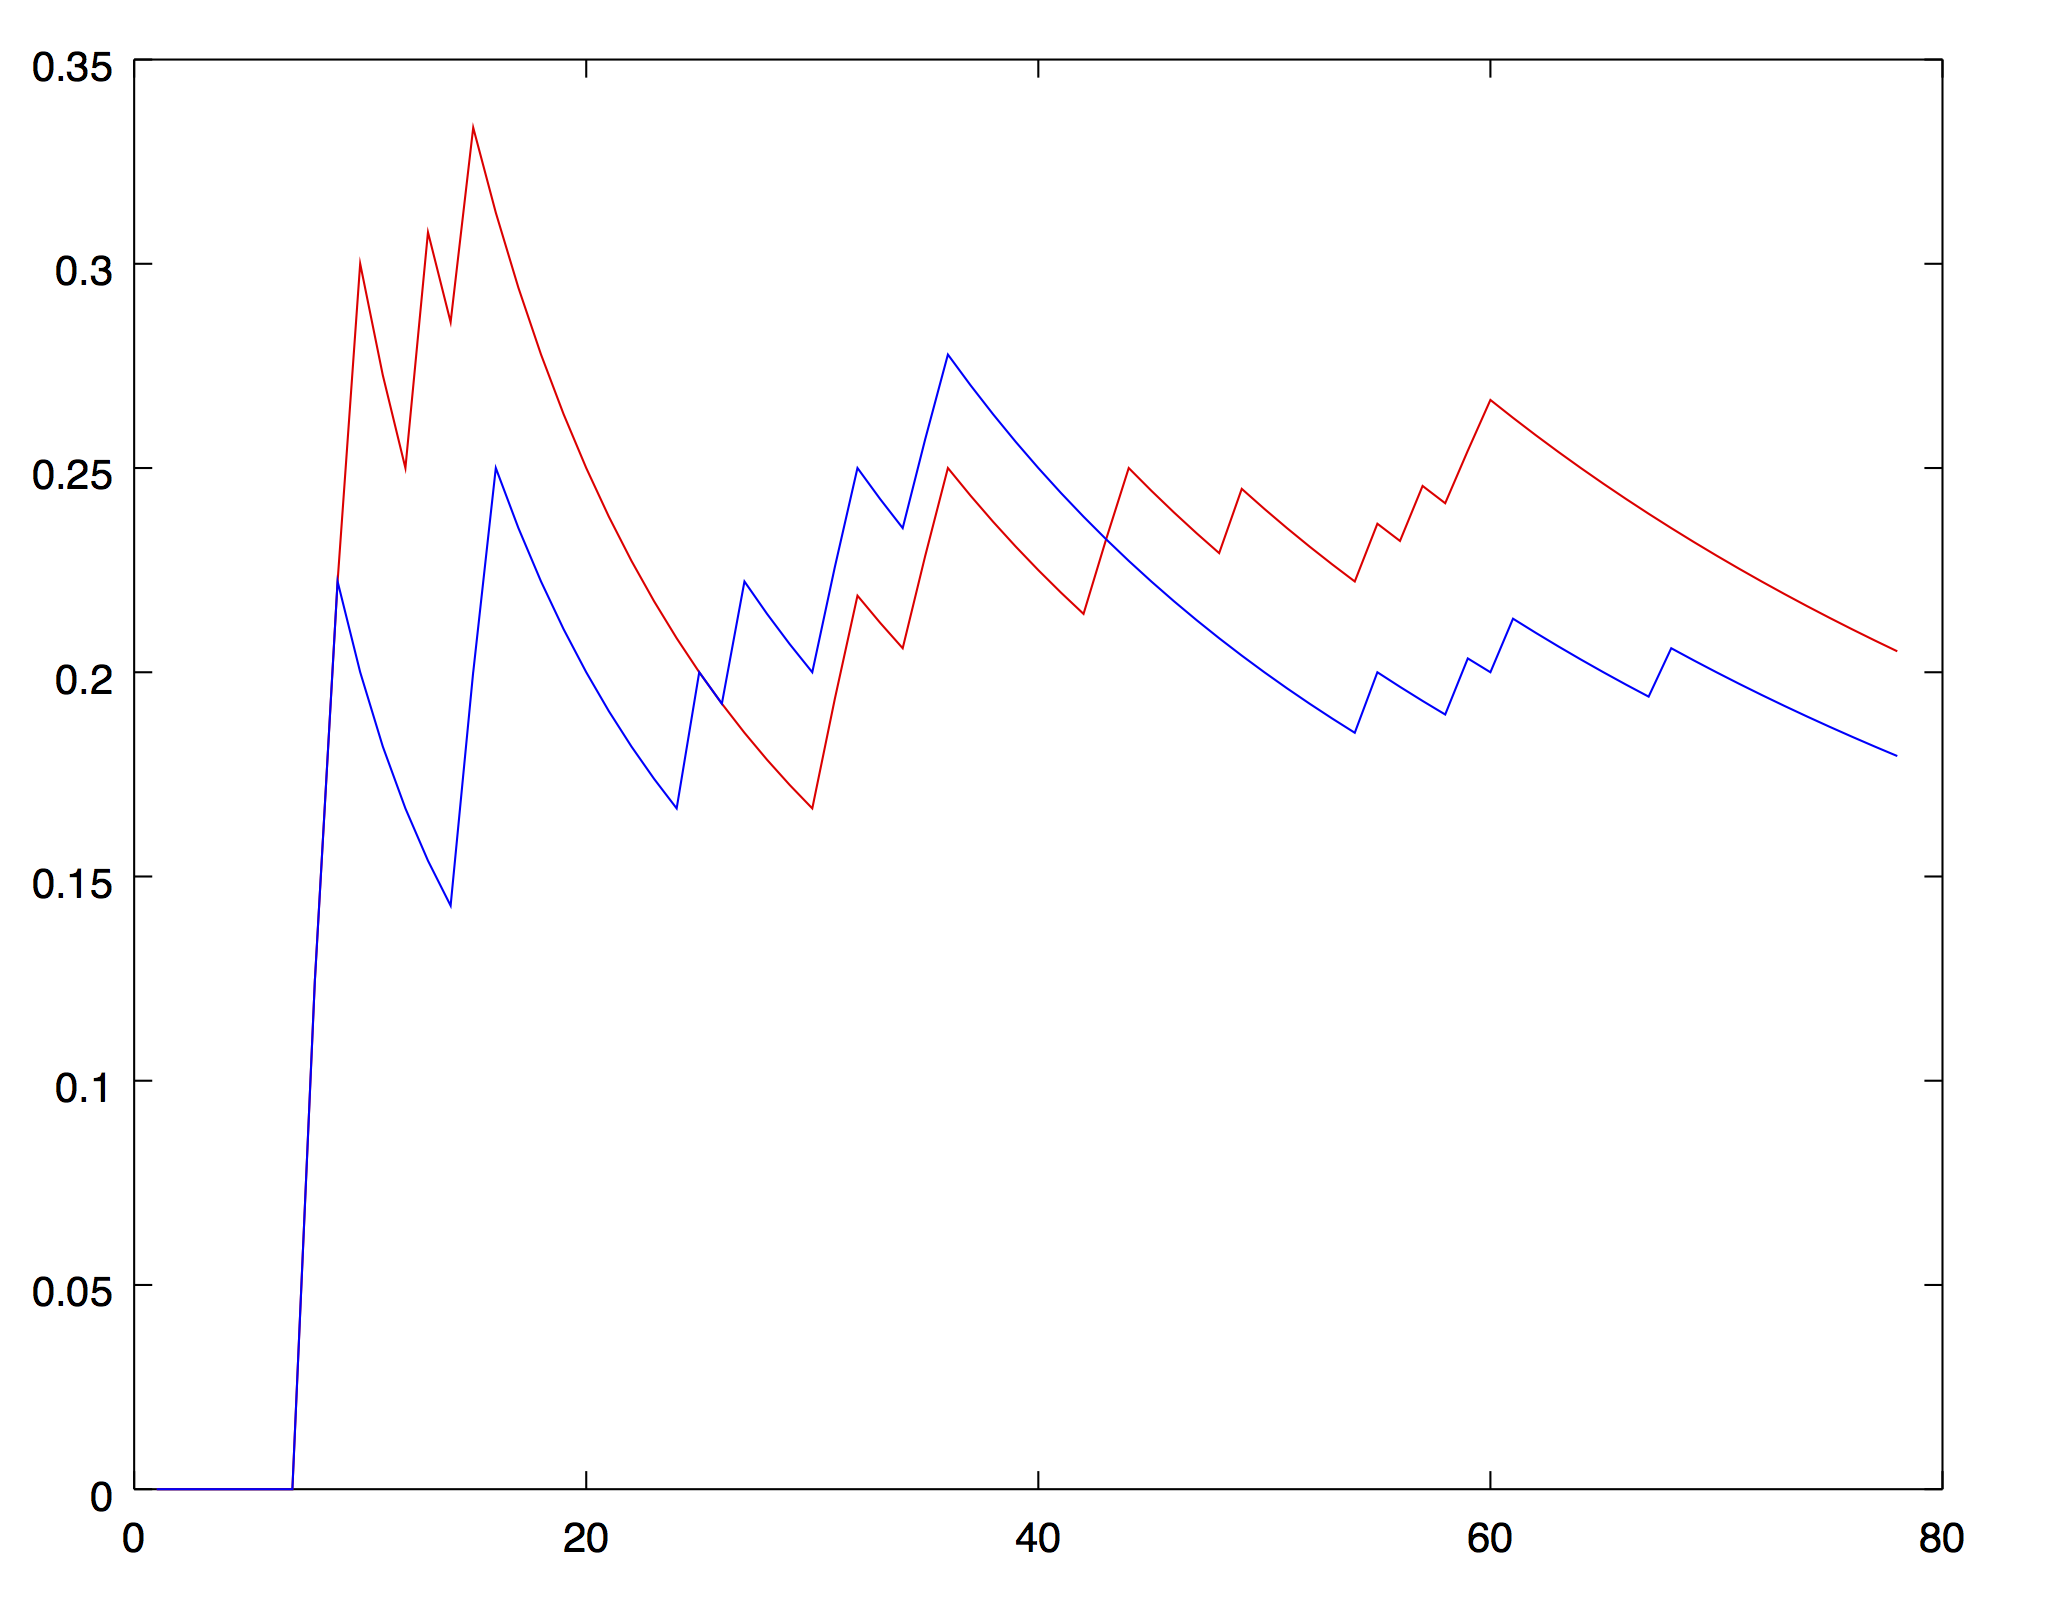
\includegraphics[width=0.9\textwidth]{chart}
			\end{center}
		\end{figure}

		\paragraph{}

%----------------------------------------------------------------------------------------
%	Bibliographic references
%----------------------------------------------------------------------------------------
  \begin{thebibliography}{9}

		\bibitem{jordan:article}
    	Jordan: Serial Order: A distributed parallel approach (1986)

		\bibitem{elman:article}
    	Elman: Finding Structure in Time (1990)

		\bibitem{financial:article}
    	Jie Wang, Jun Wang, Wen Fang, Hongli Niu: Financial Time Series Prediction Using Elman Recurrent Random Neural Networks (2016) \url{https://www.ncbi.nlm.nih.gov/pmc/articles/PMC4887655/}
	\end{thebibliography}

\end{document}
